In questo paragrafo verranno presentate due modifiche alla topologia di reti neaurali descritte nei capitoli precedenti, in particolare una modifica su rete GRU e una su rete TCN. Verranno innanzitutto presentati e spiegati singolarmente ognuno dei diversi livelli utilizzati nelle modifiche ed infine ciascuna rete interamente modificata.

% res(5) - C1BATCH (filterSize=3)	best GRU			
% res(5) - C1 (filterSize=3)	best temporal

			


\section{Livello Convoluzionale}
La convoluzione è una delle più importanti operazioni di image processing attraverso la quale si applicano filtri digitali. In questo particolare caso sono stati utilizzati dei livelli di convoluzione 1D in quanto, per come sono stati strutturati i dataset di input, questa risulta essere l'unica operazione permessa.
Un filtro digitale (piccola maschera di pesi 1D) viene fatto scorrere sulle diverse posizioni di input; per ogni posizione viene generato un valore di output ottenuto eseguendo il prodotto scalare tra la maschera e la relativa porzione di input coperta. Tale operazione, specifica per livelli convolutivi 1D, si può sintetizzare (ignorando il bias) in:
\begin{equation}
	net_{t} = \sum_{j = -\lfloor F/2 \rfloor}^{\lfloor F/2 \rfloor}w_{j} \cdot in_{t+j}
\end{equation}
dove $j$ è l'indice di un sottoinsieme del vettore di input, $w_{j}$ è il peso all'indice $j$, $F$ è la dimensione del filtro e $in_{t+j}$ il valore del vettore di input.

Per effettuare una la convoluzione spesso è necessario utilizzare altri passi e altre proprietà tipiche dell'operazione di convoluzione come Stride e Padding con lo scopo di ottimizzarne poi l'output.

\textbf{Stride} è una proprietà dell'operazione di convoluzione nella quale il filtro viene fatto scorrere sul volume di input non con passi unitari (default) ma con un passo maggiore (detto Stride). Lo \textit{Stride} riduce la dimensione delle feature map nel volume di output e conseguentemente il numero di connessioni; piccoli Stride (e.g. 2 o 4) possono aumentare l'efficienza a discapito di una leggera penalizzazione in accuratezza.

\textbf{Padding} è una proprietà dell'operazione di convoluzione che permette di regolare la dimensione delle feature map aggiungendo un bordo al volume di input (valori nulli). Con il parametro \textit{Padding} si denota lo spessore del bordo. Il Padding è utile per filtrare i pixel laterali dell'immagine; senza Padding tutti i pixel del bordo vengono analizzati da un numero molto ridotto di filtri, poichè tali filtri non possono uscire dalla matrice di input, portando dunque ad una riduzione di dimensione dell'output e ad una perdita di informazione.

Nelle modifiche effettuate il parametro di \textit{Stride} è 1 e \textit{Padding} è 'same', ovvero impostato in modo tale che la dimensione dell'output sia la stessa della dimensione dell'input quando Stride=1.

Il livello Convoluzionale viene identificato con l'id C1.

\section{Livello di Batch-Normalization}
Il livello di Batch-Normalization (BN) è un metodo che rende l'addestramento delle reti neurali profonde (DNN) molto più veloce e stabile, che permette di standardizzare l'input per ogni mini-bacth della rete. Tale operazione ha l'effetto di stabilizzare il processo di apprendimento e di ridurre drasticamente il numero di periodi di addestramento necessari per le reti neurali profonde.

La Batch-Normalization può essere implementata durante l'addestramento calcolando la media e varianza di ciascuna variabile di input per ogni mini-batch e utilizzando queste informazioni statistiche per eseguire la standardizzazione. Si ha, dunque, il calcolo della media:
\begin{equation}
	\mu_{i} = \frac{1}{m}\sum_{j=1}^{m}x_{ij}
\end{equation}
e della varianza:
\begin{equation}
	\sigma_{i}^{2} = \frac{1}{m}\sum_{j=1}^{m}(x_{ij}-\mu_{i})^{2}
\end{equation}
dove $m$ è il numero di elementi di input e $x_{ij}$ è l'input $j$-esimo relativo alla $i$-esima dimensione.

Infine, la normalizzazione diventa:
\begin{equation}
	\hat{x_{ij}} = \frac{x_{ij} - \mu_{i}}{\sqrt{\sigma_{i}^{2}+\epsilon}}
\end{equation}
dove $\epsilon=10^{-5}$.

%variabile Batch Size → Se la dimensione batch è 1, la varianza sarà 0, il che non consente il funzionamento della norma batch. Inoltre, se abbiamo mini-batch di piccole dimensioni, diventa troppo rumoroso e l'allenamento potrebbe influire. Ci sarebbe anche un problema nella formazione distribuita. Ad esempio, se stai calcolando su macchine diverse, devi prendere la stessa dimensione del batch perché altrimenti γ e β saranno diversi per sistemi diversi.
%Rete neurale ricorrente → In un RNN, le attivazioni ricorrenti di ogni fase temporale avranno una storia diversa da raccontare (cioè le statistiche). Ciò significa che dobbiamo inserire un livello di norma batch separato per ogni fase temporale. Questo rende il modello più complicato e dispendioso in termini di spazio perché ci costringe a memorizzare le statistiche per ogni passaggio temporale durante l'allenamento.


%[citazione - Batch Normalization: Accelerating Deep Network Training by Reducing Internal Covariate Shift]

Il livello di Batch Normalization viene identificato con l'id BN.

\section{Modifica della topologia su rete GRU}
In questa modifica sono stati utili utilizzati un livello Convoluzionale e un livello di Batch-Normalization, inseriti subito prima della rete GRU base.

Il motivo per cui è stato aggiunto un livello di convoluzione è che un'operazione come la convoluzione stessa permette di effettuare una limatura del valore della feature di ingresso con i valori limitrofi delle feature. Queste piccole modifiche locali possono aiutare a raggiungere una maggiore indipendenza spaziale, aiutando la generalizzazione del modello.

Successivamente è stato inserito un livello di Batch-Normalization con lo scopo di rendere il sistema più veloce e stabile, attraverso la normalizzazione dei valori di input alla rete.

\vspace{0.25cm} 
\begin{center}
	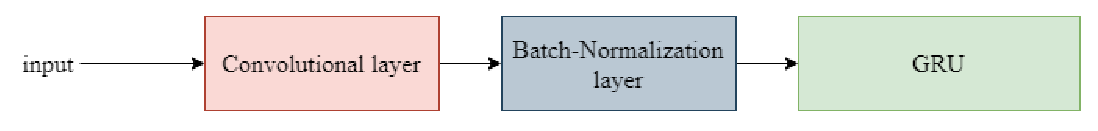
\includegraphics[scale=0.8]{images/gru.eps}
	\captionof{figure}{Schema della rete GRU-C1BN}
	\label{Figura 1.}
\end{center}
\vspace{0.25cm}


\section{Modifica della topologia su rete TCN}
In questa modifica è stato utilizzato un solo livello Convoluzionale inserito subito prima della rete TCN base.

I motivi per cui è stato aggiunto un livello di convoluzione sono gli stessi detti in precedenza: tale livello permette il raggiungimento di una indipendenza spaziale e ciò aiuta il sistema a generalizzare meglio il modello, cosa fondamentale se si vogliono aumentare le performance della rete.
\vspace{0.25cm} 
\begin{center}
	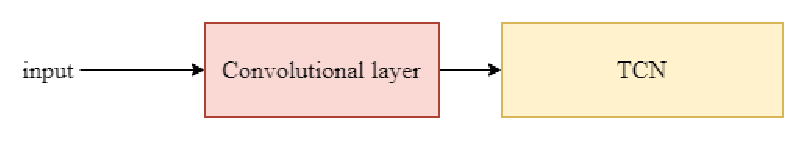
\includegraphics[scale=0.8]{images/tcn.eps}
	\captionof{figure}{Schema della rete TCN-C1}
	\label{Figura 1.}
\end{center}
\vspace{0.25cm}
